\chapter{Model checker}\label{ch:ch2}

В этой главе мы разберем устройство реализованного \autocite{CheckerRepo} model checker-а.

\section{Управление исполнением}

Чтобы перебирать состояния исполнения, нужно:

\begin{itemize}
\item	делать снимки текущего состояния исполнения в точках обращения к примитивам синхронизации / атомикам;

\item	восстанавливать это состояние из снимка;

\item	управлять очередностью исполнения потоков (управлять планировщиком).
\end{itemize}

Для этого будем пользоваться \emph{файберами} – кооперативными потоками, реализованными в пространстве пользователя. По сути, мы продублируем в пространстве пользователя всю механику исполнения из ядра операционной системы: управление очередью исполнения и очередями ожидания в примитивах синхронизации, процедуру переключения контекста исполнения и т.п.

Файберы исполняются в одном потоке операционной системы, что исключает влияние на моделируемое исполнение недетерминизма системного планировщика.

Файбер хранит в себе:

\begin{itemize}

\item	Стек – заранее аллоцированный регион памяти.

\item	Контекст – callee-saved регистры, instruction pointer, stack pointer (имеет смысл только для остановленного файбера).

\item	Enum состояния: файбер готов исполняться (\mintinline{c++}{runnable}) / заснул в очереди ядра (\mintinline{c++}{suspended}) / завершил исполнение (\mintinline{c++}{terminated}).

\item	Пользовательскую функцию.

\end{itemize}

Переключение контекста файбера реализовано на ассемблере и состоит из следующих шагов:

\begin{enumerate}

\item	На стек файбера сохраняется контекст исполнения: значения callee-saved регистров.

\item	\mintinline{c++}{rsp} текущего файбера фиксируется в поле файбера для восстановления контекста в будущем.

\item	\mintinline{c++}{rsp} переключается на стек нового файбера.

\item	С нового стека восстанавливается контекст (значения callee-saved регистров).

\end{enumerate}

Таким образом, в файбере в поле с контекстом фактически хранится лишь указатель \mintinline{c++}{rsp}, остальные регистры хранятся на стеке.

\textbf{Замечание:} в работе мы будем использовать термин \emph{файберы}, когда речь идет о реализации model checker-а, и \emph{потоки}, когда речь идет о наблюдаемом поведении теста / свойствах конкурентных исполнений. Пользователь model checker-а работает только с потоками (через объект \mintinline{text}{thread}) и никаких файберов не наблюдает.


\section{Снимки состояния}

Состояние исполнения образовано:

\begin{itemize}
\item	состоянием каждого файбера (стек, регистры, enum состояния, исполняемая функция);

\item	состоянием динамической памяти (кучи).
\end{itemize}

Снимок состояния делается в контексте model checker-а, т.е. в момент, когда ни один из файберов не исполняется.

Снимок регистров отдельно делать не нужно: при переключении контекста нужные регистры сохраняются на вершину стека остановленного файбера, так что достаточно сохранять только сами стеки.

Сохраняется только использованная часть стека – до адреса \mintinline{c++}{rsp} (он доступен через сохраненный контекст исполнения).

Между стеками файберов / стеком и кучей могут быть ссылки, про которые model checker ничего не знает (один файбер захватывает мьютекс, который расположен на стеке другого файбера / файбер создает \mintinline{c++}{shared_ptr} на объект), поэтому память для стеков и кучи выделяется в model checker-е один раз, и при каждом восстановлении снимка стеки и куча восстанавливаются по своим прежним адресам. 

Все аллокации в тесте перехватываются, и если аллокация выполняется непосредственно пользовательским кодом (а не model checker-ом), то ее обрабатывает специальный аллокатор. Аллокатор поддерживает свободные блоки в интрузивном односвязном списке внутри заранее выделенной арены памяти. Снимок аллокатора – это использованный диапазон арены и два указателя: на голову списка свободных блоков и на границу использованного префикса арены.

Служебные аллокации, выполняемые в контексте файбера (например, при запуске нового потока-файбера), отделяются от пользовательских аллокаций с помощью расставленных в библиотеке \mintinline{c++}{AllocationGuard}-ов. \mintinline{c++}{AllocationGuard} выключает аллокатор model checker-а в области своей жизни.

Итого, снимок состояния в model checker-е образован:

\begin{itemize}
\item	стеком, enum-ом состояния и исполняемой функцией каждого файбера;

\item	снимком кучи.
\end{itemize}

\begin{figure}
	\centerfloat{
		
		
					\begin{tabular}{c c c}
						%\centering 
						\fbox{{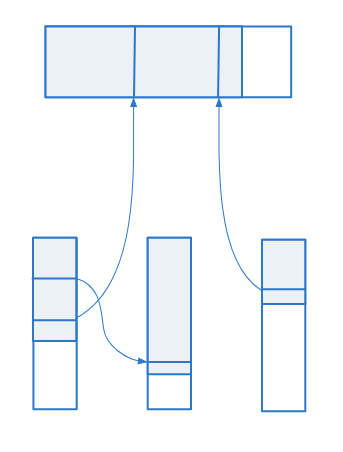
\includegraphics[align=c,width=0.35\textwidth]{snap1}}}
						&
						${\Longrightarrow}$
						& \fbox{{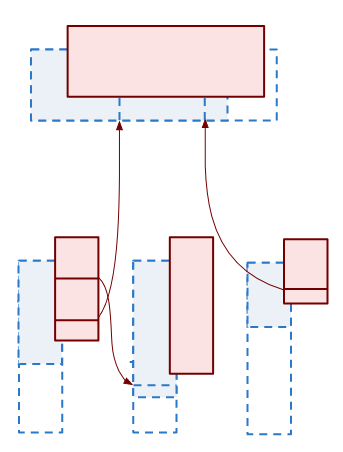
\includegraphics[align=c,width=0.35\textwidth]{snap2}}}
						\\
						\hfil Память (куча и стеки) & & \hfil Снимок
					\end{tabular}
			
	}
	\bigskip
	\caption{Снятие снимка состояния.}
\end{figure}

\section{Перебор исполнений}

Чтобы находить кратчайшие нарушения инвариантов, будем обходить граф состояний исполнения поиском в ширину. Граф не материализуется в памяти явно, вместо этого мы умеем из каждого состояния получать все смежные с ним.

\subsection{Обход графа состояний}

Посмотрим, как model checker перебирает исполнения теста.

Ключевой объект model checker-а – это очередь состояний, продолжения которых еще нужно посетить, фронт обхода в ширину. 

На старте model checker создает первый файбер, который будет исполнять код теста, и кладет снимок начального состояния в очередь.

Теперь посмотрим на цикл обхода графа состояний. На очередной итерации model checker достает из очереди снимок состояния, перебирает все файберы, которые в этом состоянии могут продолжить работу, и для каждого из них исполняет один \emph{шаг} (\mintinline{c++}{Step}). 

\iftoggleverb{pics}

\begin{figure}
	\centerfloat{
		\fbox{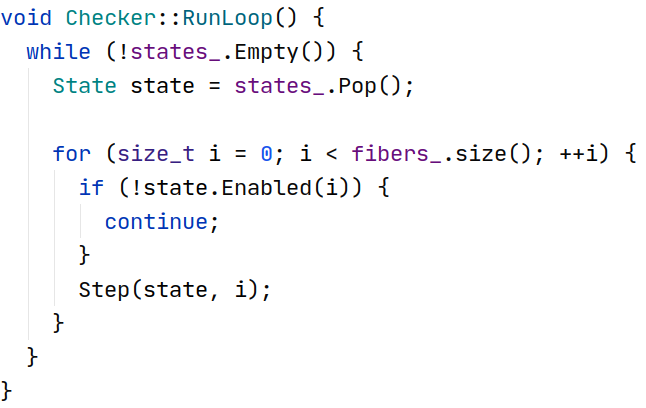
\includegraphics[scale=0.5]{runloop}}
	}
	\bigskip
	\caption{Цикл model checker-а.}\label{fig:runloop}
\end{figure}

\else

\begin{listing}
	\centering
	
	\begin{minted}{c++}
void Checker::RunLoop() {
	while (!states_.Empty()) {
		State state = states_.Pop();

		const size_t fiber_count = fibers_.size();
		for (size_t i = 0; i < fiber_count; ++i) {
			if (!state.Enabled(i)) {
				continue;
			}
			Step(state, i);
		}
	}
}
	\end{minted}
	\caption{Цикл model checker-а.}
	\label{loop}
\end{listing}

\fi

Перебор \mintinline{c++}{runnable} файберов для каждого снимка – это и есть ветвление исполнения, по сути мы рандомизируем run queue в планировщике.

\subsection{Шаг исполнения}

Шаг исполнения файбера заключен между точками обращения к разделяемым объектам (примитивам синхронизации / атомикам / аллокатору памяти) и реализуется парой служебных функций \mintinline{c++}{Step} / \mintinline{c++}{Fork}.

Начинается шаг с вызова функции \mintinline{c++}{Step}: в контексте model checker-а из снимка восстанавливается состояние исполнения (куча и стеки накладываются на соответствующие регионы памяти), затем контекст переключается на выбранный файбер (который ранее остановился в вызове \mintinline{c++}{Fork}).

Далее файбер исполняется до тех пор, пока не встретит следующий вызов функции \mintinline{c++}{Fork}.

\iftoggleverb{pics}

\begin{figure}
	\centerfloat{
		\fbox{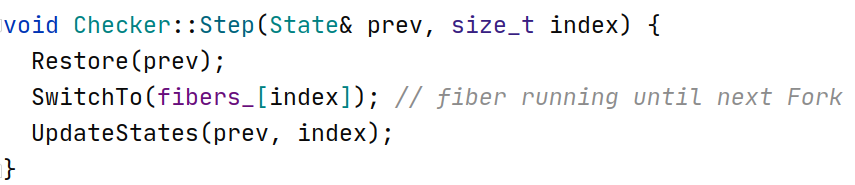
\includegraphics[scale=0.4]{step}}
	}
	\bigskip
	\caption{Шаг файбера (\mintinline{c++}{Step}).}\label{fig:step}
\end{figure}

\else

\begin{listing}
	\centering
	
	\begin{minted}{c++}
    
void Checker::Step(State& prev, size_t index) {
  Restore(prev);
  SwitchTo(fibers_[index]);
  // fiber running until next Fork...
  UpdateStates(prev, index);
}

	\end{minted}
	\caption{Шаг файбера (\mintinline{c++}{Step}).}
	\label{step}
\end{listing}

\fi

Вызов \mintinline{c++}{Fork} – точка ветвления, в ней может произойти переключение на произвольный \mintinline{c++}{runnable} файбер. Вызов \mintinline{c++}{Fork} переключает контекст файбера на контекст model checker-а, тот делает снимок состояния исполнения и помещает его в очередь поиска в ширину.

\begin{figure}
	\centerfloat{
		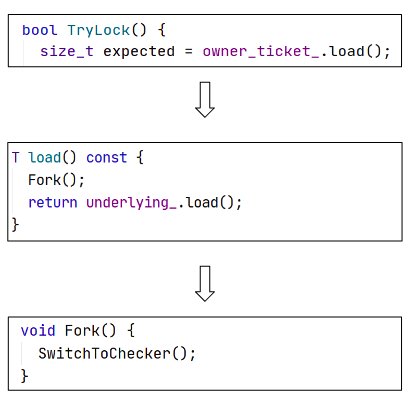
\includegraphics[scale=0.5]{forkblack}
	}
	\caption{Развилка в коде (вызов \mintinline{c++}{Fork}).}\label{fig:fork}
\end{figure}

\subsection{Точки ветвления}

Будем предполагать, что реализация верифицируемого конкурентного объекта не содержит data race-ов, т.е. проверяемый тест – программа, \emph{свободная от гонок (data-race-free)}. 

Если программа свободна от гонок, то потоки в ней не могут наблюдать относительный порядок действий между точками синхронизации в другом потоке (т.е. между обращениями к атомикам, мьютексам и другим объектам, через которые реализуется отношение synchronizes-with).

Это наблюдение упрощает перебор model checker-а: ветвления исполнения (вызовы \mintinline{c++}{Fork}) можно встраивать только при обращении к объектам, через которые осуществляется синхронизация.

Чтобы перехватывать обращения к атомикам, мьютексам и условным переменным и ветвить в них исполнения, мы пишем собственные версии этих примитивов и требуем от пользователя model checker-а, чтобы он использовал их вместо стандартных (для этого в проверяемом коде придется заменить пространство имен с \mintinline{c++}{std} на пространство имен библиотеки model checker-а, на данный момент это \mintinline{c++}{twist::stdlike}).

\iftoggleverb{pics}

\begin{figure}
	\centerfloat{
		\fbox{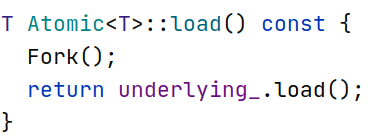
\includegraphics[scale=0.5]{load}}
	}
	\bigskip
	\caption{Собственная реализация \mintinline{c++}{load} у атомика.}\label{fig:lock}
\end{figure}

\else

\begin{listing}
	\centering
	
	\begin{minted}{c++}
    
void Mutex::Lock() {
  Fork();
  while (locked_) {
    wait_queue_.Park();
  }
  locked_ = true;
}

	\end{minted}
	\caption{Реализация метода lock у мьютекса.}
	\label{lock}
\end{listing}

\fi

Аналогично, для перехвата динамических аллокаций мы переопределяем операторы \mintinline{text}{new} / \mintinline{text}{delete}: если находимся в контексте пользовательского кода, вызываем аллокатор model checker-а, иначе – \mintinline{c++}{malloc} / \mintinline{c++}{free}.

\subsection{Run queue / Wait queue}

Model checker – не планировщик, в нем нет явной очереди \mintinline{c++}{runnable} файберов (run queue), для каждого снимка запускается каждый \mintinline{c++}{runnable} файбер. 

Аналогично мы поступаем с блокирующими примитивами синхронизации, которые внутри имеют очереди ожидания (мьютексы, условные переменные): 

Явно такие очереди не моделируются, вместо этого в каждом файбере хранится адрес очереди, в которой он заснул. Когда, например, мьютекс в \mintinline{c++}{unlock} будит один из заблокированных на нем файберов, model checker создает сразу несколько веток исполнения – по ветке на каждый файбер, у которого в поле адреса хранится текущая очередь.

В планировщике Go \autocite{Go} при поиске гонок происходит рандомизация очередей ожидания и исполнения. У нас же случайность трансформируется в перебор всех возможных исполнений.


\subsection{Очередь во внешней памяти}

С ростом исследуемой глубины исполнения количество состояний будет расти экспоненциально, фронт поиска в ширину быстро станет огромным (в одном из тестов размер фронта достигал десятков миллионов состояний) и перестанет помещаться в оперативную память.

Поэтому очередь для поиска в ширину в model checker-е реализована во внешней памяти. Вот как она устроена:

Все состояния в очереди делятся на две непрерывные группы (фронта):

\begin{enumerate}

\item	\emph{Старый фронт} – состояния наименьшей глубины ($d$). 

\item	\emph{Новый фронт} – состояния, полученные из старого фронта (глубины $d+1$). 

\end{enumerate}
	
Пока не исчерпался старый фронт, в очереди не могут появиться состояния глубины $d+2$.
 
Будем поддерживать по файлу на каждый из двух фронтов: один для чтения старого фронта, другой – для записи нового. При смене глубины старый фронт отбрасывается, а новый – переходит в старый. 

Model checker не работает с файлами напрямую, вместо этого он использует специальный аллокатор, который работает с аренами памяти, отображенными в файлы с помощью \mintinline{c++}{mmap}-а.

Максимальный перерасход внешней памяти (в два раза) происходит при смене глубины. Но почти всегда издержки компенсируются (если следующий фронт произведет хотя бы в два раза больше состояний).


\subsection{Повторные состояния}

Чтобы не посещать одни и те же состояния повторно, model checker хеширует снимки состояний и не помещает снимок в очередь, если его хеш уже встречался ранее.

Хеширование неизбежно ведет к потере информации, поэтому model checker может упустить состояния, если произойдет \emph{коллизия} – ситуация, когда двум состояниям ставится в соответствие один хеш. 

TLC аналогичным образом использует хеширование состояний. Кроме того, он оценивает вероятность коллизии и дает возможность пользователю перезапустить перебор с другой хеш-функцией:

“TLC saves only 64-bit fingerprints (hashes) of the reachable states that it finds, not the complete states.  If two different reachable states have the same fingerprint, a situation called a collision, TLC may not find all reachable states.  At the end of a run, TLC prints estimates of how likely it was that a collision occurred.” \autocite{TlcOptions}

\begin{figure}
	\centerfloat{
		\fbox{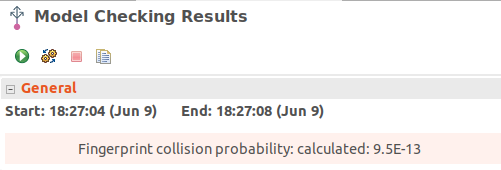
\includegraphics[scale=0.5]{fingerprint}}
	}
	\bigskip
	\caption{Вероятность коллизии, показанная в TLA+ Toolbox.}\label{fig:fingerprint}
\end{figure}

Но вероятность коллизии невелика, и на практике хеширование не мешает model checker-у находить баги, зато сильно ускоряет проверку. 

Для хеширования model checker использует FNV-функцию \autocite{Fnv}: она быстрая и обобщается на комбинирование хешей (что удобно для хеширования состояний исполнения).
  
При хешировании участков памяти (стеки, куча) помогает развертка цикла \autocite{FasterHash}. Развертка разрывает зависимость следующей итерации цикла от предыдущей, и процессор (фактически, конвейер для инструкций) выполнит такие итерации параллельно.

\section{Симметрия}

Любой model checker сталкивается с проблемой \emph{state space explosion}. Даже если разветвляться только перед обращениями к разделяемым объектам, количество состояний будет расти экспоненциально с ростом количества атомиков / потоков. 

Но если разные потоки исполняют один и тот же код (что ожидаемо для теста мьютекса или конкурентной структуры данных), то некоторые состояния могут быть \emph{симметричны} – сводиться одно к другому с помощью перенумерации потоков. 

Чтобы учесть симметрию, model checker \emph{канонизирует} состояние: стирает со стеков зависимости от адреса конкретного потока (например, ссылки на свой же стек заменяет относительными отступами). Получившиеся стеки хешируются по отдельности, сортируются и комбинируются в один результирующий хеш.

TLC тоже предоставляет такую оптимизацию и обобщает это наблюдение до симметрии множеств \autocite{Symmetry}.

\section{Проверка инвариантов}

Цель model checker-а – найти нарушение инварианта в некотором исполнении теста или убедиться в отсутствии таких нарушений во всех исполнениях.

Есть две вариации инвариантов:

\begin{itemize}

\item	Локальный инвариант – аналог обычного assert-а, задается в коде теста макросом \mintinline{c++}{CHECKER_ASSERT(condition)}. Проверка выполняется в контексте пользовательского потока. Если \mintinline{c++}{condition} не выполнен, то управление передается model checker-у, и тот сообщает об ошибке. 

\item	Глобальный инвариант – произвольный предикат на разделяемом состоянии. Инвариант проверяется в контексте model checker-а: проверка запускается на каждое новое состояние в исполнении и происходит атомарно (с отключенными \mintinline{c++}{Fork}-ами). Глобальный инвариант задается в начале теста с помощью \mintinline{c++}{AddInvariant(predicate)}.

\end{itemize}

Для проверки взаимного исключения в мьютексе удобнее поставить \mintinline{c++}{CHECKER_ASSERT} в критической секции: 

\iftoggleverb{pics}

\begin{figure}
	\centerfloat{
		\fbox{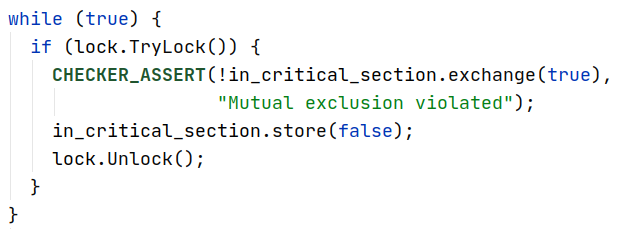
\includegraphics[scale=0.5]{checkerassert}}
	}
	\bigskip
	\caption{Локальный инвариант.}
\end{figure}

\else

\begin{listing}
	\centering
	
	\begin{minted}{c++}
    
while (true) {
  if (lock.TryLock()) {
    CHECKER_ASSERT(!in_critical_section.exchange(true), "Mutual exclusion violated");
    in_critical_section.store(false);
    lock.Unlock();
  }
}

	\end{minted}
	\caption{Локальный инвариант.}
	\label{local}
\end{listing}

\fi

Но инварианты lock-free стека уже трудно проверить локально, для него удобнее использовать глобальный вариант (например, он может проверять, что каждый узел стека действительно аллоцирован (см. \ref{app:A3})):

\iftoggleverb{pics}

\begin{figure}
	\centerfloat{
		\fbox{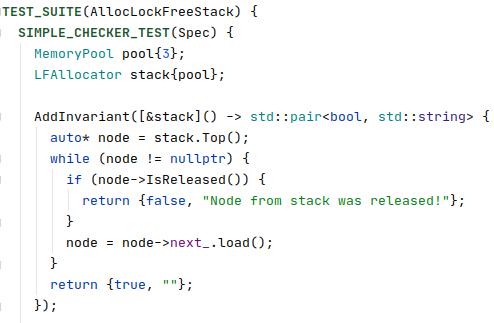
\includegraphics[scale=0.7]{globalassert}}
	}
	\bigskip
	\caption{Глобальный инвариант.}
\end{figure}

\else

\begin{listing}
	\centering
	
	\begin{minted}{c++}

TEST_SUITE(AllocLockFreeStack) {
  SIMPLE_CHECKER_TEST(Spec) {
    MemoryPool pool{3};
    LFAllocator stack{pool};
        
    AddInvariant([&stack]() -> std::pair<bool, std::string> {
      // check every node of stack...
      // validation failed -> return {false, report}
    });
	
    // test code...
  }
}
	\end{minted}
	\caption{Глобальный инвариант.}
	\label{localinv}
\end{listing}

\fi

В model checker-е реализован глобальный служебный инвариант – проверка \emph{взаимной блокировки (deadlock)}. Взаимная блокировка с точки зрения model checker-а – достижимое состояние, в котором еще есть живые потоки, но нет ни одного потока, готового исполняться (т.е. в состоянии \mintinline{c++}{runnable}). Как и TLC, model checker проверяет этот инвариант по умолчанию.  


\section{Печать траектории}

Если при проверке теста model checker находит состояние, в котором нарушается пользовательский или служебный инвариант, то он завершает перебор и печатает найденную траекторию. Пример найденной траектории приведен в приложении \ref{app:trace}.

Проверка инварианта и печать траектории разделены между двумя режимами сборки теста: \mintinline{c++}{Check} и \mintinline{c++}{Trace}.

В режиме \mintinline{c++}{Check} model checker обходит граф состояний исполнения и с каждым снимком состояния хранит траекторию, которая привела к этому состоянию. Траектория детерминирует выбор очередного потока в каждой развилке исполнения и кодируется последовательностью индексов потоков: на $i$-ой позиции записан номер потока, который был выбран на $i$-ом вызове \mintinline{c++}{Fork}. В случае нарушения инварианта найденная траектория сохраняется на диск.

В режиме \mintinline{c++}{Trace} model checker считывает с диска найденную в первом режиме траекторию и проигрывает ее, показывая для каждой развилки разделяемое состояние, стеки потоков и локальные переменные.  

Траектория разделена на секции (\emph{runs}), каждая секция – непрерывный фрагмент исполнения одного потока, который ограничен переключением контекста / стартом потока (слева) / завершением потока (справа).

Каждая секция показывает состояние потока в нескольких временных точках: снимки состояния до и после исполнения секции, и промежуточные снимки в точках обращения к атомикам / примитивам синхронизации / аллокатору памяти.

Для каждого шага в секции печатается:

\begin{itemize}
\item	Разделяемое состояние. Model checker не знает, как устроено и как печатать разделяемое состояние, пользователь пишет процедуру печати самостоятельно и через \mintinline{c++}{PrintState} в начале теста передает ее model checker-у.

\begin{figure}
	\centerfloat{
		\fbox{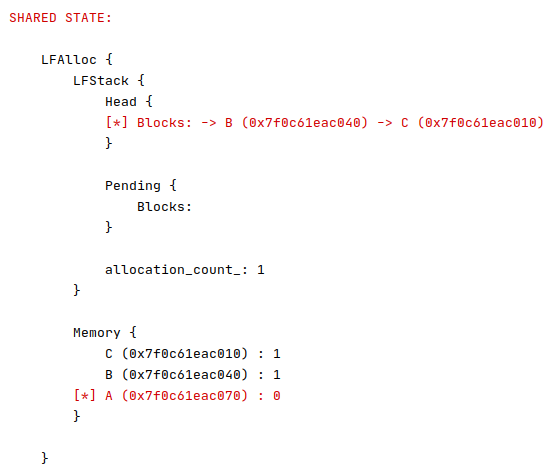
\includegraphics[scale=0.5]{sharedstate}}
	}
	\bigskip
	\caption{Разделяемое состояние.}
\end{figure}

\item	Стектрейсы потока. Стектрейсы собираются с помощью библиотеки \mintinline{c++}{backward-cpp} \autocite{Backward}. Служебные фрагменты стектрейса (вызовы внутри model checker-а), код стандартной и сторонних библиотек фильтруется.

\item	Локальные переменные. В точке, где мы хотим снять значения локальных переменных, мы вызываем \mintinline{c++}{fork} и из дочернего процесса присоединяемся отладчиком (\mintinline{c++}{gdb}) к родительскому. В планах – использовать программный интерфейс \mintinline{c++}{lldb} вместо запуска дебаггера.

\begin{figure}
	\centerfloat{
		\fbox{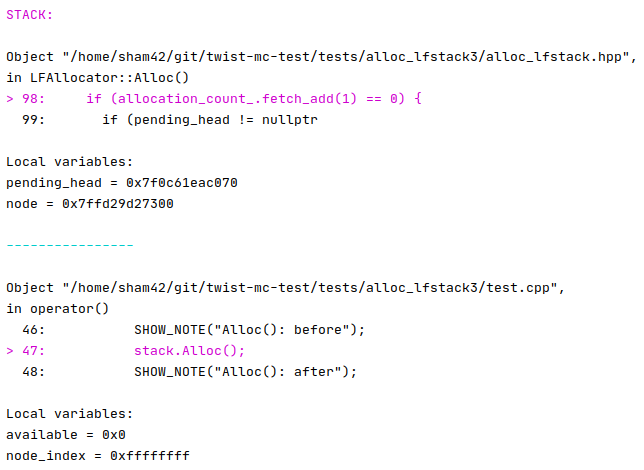
\includegraphics[scale=0.5]{stacklocals}}
	}
	\bigskip
	\caption{Стектрейсы и локальные переменные.}
\end{figure}

\item	Заметки о служебных событиях во время исполнения потока. Добавляются с помощью макроса \mintinline{c++}{SHOW_NOTE}.

\begin{figure}
	\centerfloat{
		\fbox{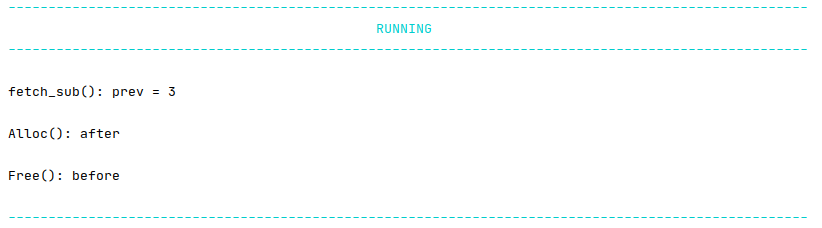
\includegraphics[scale=0.5]{running}}
	}
	\bigskip
	\caption{Заметки о событиях.}
\end{figure}

\end{itemize}

\section{Инженерные препятствия}

Model checker проверяет код, оптимизируемый компилятором. Поэтому нужно решать ряд трудностей, связанных непосредственно с языком программирования / оптимизациями компилятора.

\subsection{Абсолютные адреса и симметрия}

Для учета симметрии model checker канонизирует стеки, но этому процессу мешают абсолютные адреса:

\begin{itemize}
\item	При вызове функции на стек сохраняется указатель на начало родительского фрейма (значение регистра \mintinline{c++}{rbp}).

\item	На стеке может лежать ссылка на переменную, аллоцированную на этом стеке (в виде другой переменной или в виде значения регистра).

\item	В вызове \mintinline{c++}{Fork} перед переключением на контекст model checker-а вызывается служебная функция \mintinline{c++}{GetCurrentFiber}. В результате на стеке может “отпечататься” адрес текущего файбера.

\item	Файбер хранит исполняемую лямбду в type-erased контейнере. Для механизма type erasure требуется аллокация на куче. Так как такая аллокация происходит независимо для каждого файбера, все контейнеры получат свой собственный уникальный адрес в памяти, даже если отвечают одной лямбде. 
\end{itemize}

Канонизация очищает стек от внутренней адресации, адреса текущего файбера и адреса контейнера для исполняемой пользовательской функции.

Это только эвристика: model checker не может отличить адрес от числа, попавшего в тот же диапазон. Но на практике такие числа редко используются программой, и model checker находит баги.

\subsection{Встраивание вызовов}

Еще одна проблема – учет одинаковых состояний в бесконечных циклах. Бесконечные циклы возникают естественным образом: например, в тесте мьютекса поток в таком цикле захватывает и отпускает мьютекс.

Ожидается, что на каждой итерации стек файбера будет отличаться только состоянием локальных переменных, объявленных перед циклом. Поэтому граф состояний исполнения должен быть небольшим. 

Рассмотрим проблему на вышеупомянутом примере (захват и освобождение мьютекса в бесконечном цикле). Компилятор может встроить вызов \mintinline{c++}{lock} в итерацию цикла. Тогда инструкции \mintinline{c++}{lock}-а “засорят” регистры в фрейме цикла. В начале следующей итерации, когда вызовется \mintinline{c++}{Fork}, “мусорные” значения callee-saved регистров сохранятся на стеке – model checker сделает снимок формально другого состояния.

Но по сути поток вернулся к тому же состоянию, с которого начинал. Если бы вызов не встроился в цикл, то метод \mintinline{c++}{lock} на выходе восстановил бы значения тех callee-saved регистров, которыми пользовался. Значит, на следующей итерации при вызове \mintinline{c++}{Fork} на стек сохранились бы те же значения регистров, что и на предыдущей. Новое состояние бы не создалось.

Есть два решения проблемы:

\begin{itemize}
\item	Вместо цикла указать в конце итерации \mintinline{c++}{RestartFiber()} – служебную функцию model checker-а, которая полностью очищает стек и перезапускает исполняемую файбером функцию. Подходит только если между итерациями на стеке не сохраняется промежуточных переменных. 

\item	Запретить компилятору “засорять” фрейм цикла: поставить вызываемым из цикла методам атрибут \mintinline{c++}{noinline}.
\end{itemize}

\subsection{Выравнивание стека}

По ABI стек должен быть выровнен перед исполнением инструкции \mintinline{asm}{call}. Чтобы это сделать, компилятору выгоднее не двигать \mintinline{c++}{rsp} напрямую, а подвинуть \mintinline{c++}{rsp} с помощью \mintinline{asm}{push %rax} \autocite{Align}. Такой \mintinline{asm}{push} совершается с регистром, в котором хранится возвращаемое значение. Поэтому, даже если цикл использует только \mintinline{c++}{noinline}-функции, вызовы таких функций могли оставить на стеке следы результата предыдущей итерации. 

Решение – заставить компилятор выравнивать стек консервативно через атрибут \mintinline{c++}{force_align_arg_pointer}. Он служит для других целей, но подошел и для нашей – компилятор для функций с таким атрибутом будет изменять \mintinline{c++}{rsp} напрямую.

